\documentclass[12pt,openright,oneside,a4paper,english,brazil]{abntex2}
\usepackage[T1]{fontenc}
\usepackage[utf8]{inputenc}
\usepackage[alf]{abntex2cite}
\usepackage{lmodern,indentfirst,microtype,amsmath,amsfonts,amssymb,graphicx,xurl,xcolor,hyperref,booktabs}
\usepackage{tikz}
\usetikzlibrary{positioning,arrows.meta}

\titulo{Fluxo Funcional do Simulador BI-AWGN}
\autor{Willian Vinícius Oliveira Araújo}
\local{Campina Grande, PB, Brasil}
\data{Outubro de 2026}
\instituicao{
 Universidade Federal de Campina Grande (UFCG)
 \par
 Unidade Acadêmica de Engenharia Elétrica (UAEE)}
\tipotrabalho{Documentação Técnica -- PIBITI}
\preambulo{Documentação do fluxo elementar de mapeamento, canal com ruído e detecção no projeto PIBITI.}

\definecolor{blue}{RGB}{41,5,195}
\makeatletter
\hypersetup{
 pdftitle={\@title},
 pdfauthor={\@author},
 pdfsubject={PIBITI - Reconciliação da informação em CV-QKD},
 pdfcreator={LaTeX with abnTeX2},
 pdfkeywords={PIBITI, CV-QKD, BI-AWGN, reconciliação},
 colorlinks=true,
 linkcolor=blue,
 citecolor=blue,
 filecolor=magenta,
 urlcolor=blue,
 bookmarksdepth=4
}
\makeatother
\setlength{\parindent}{1.3cm}
\setlength{\parskip}{0.2cm}
\begin{document}
\selectlanguage{brazil}
\frenchspacing
\imprimircapa
\textual

\chapter{Objetivo e delimitação}
Descrever a cadeia elementar de geração de bits, mapeamento antipodal, passagem por canal BI-AWGN, detecção e cálculo de BER. Trata-se de uma base didática e computacional para os futuros módulos de reconciliação; o fluxo não implementa a reconciliação multidimensional completa nem um decodificador LDPC.

\chapter{Diagrama funcional}
\begin{center}
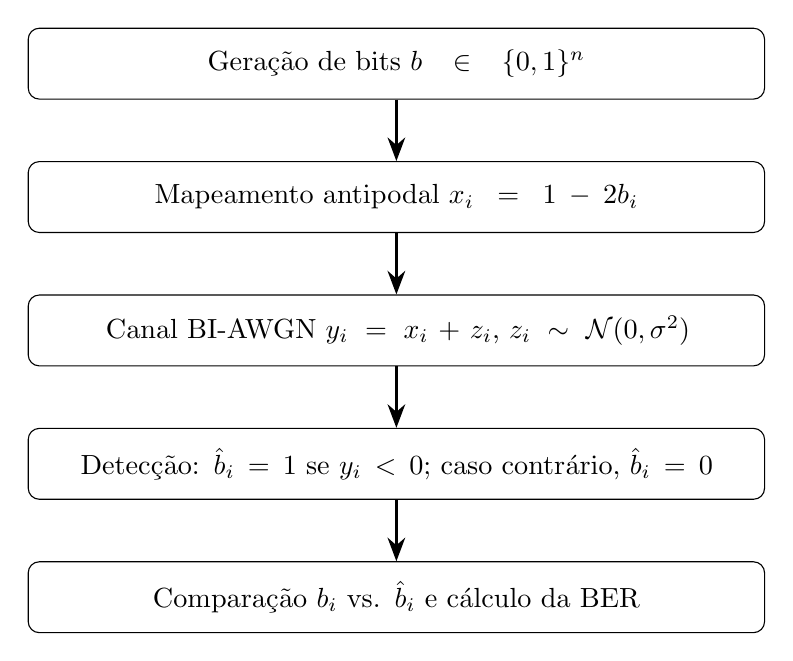
\begin{tikzpicture}[
    node distance=0.78cm,
    bloco/.style={draw,rounded corners,align=center,text width=9cm,minimum height=0.9cm,inner sep=5pt},
    seta/.style={-{Stealth[length=3mm]},thick}
]
\node[bloco] (fonte) {Geração de bits $b\in\{0,1\}^n$};
\node[bloco,below=of fonte] (map) {Mapeamento antipodal $x_i=1-2b_i$};
\node[bloco,below=of map] (canal) {Canal BI-AWGN $y_i=x_i+z_i$, $z_i\sim\mathcal N(0,\sigma^2)$};
\node[bloco,below=of canal] (det) {Detecção: $\hat b_i=1$ se $y_i<0$; caso contrário, $\hat b_i=0$};
\node[bloco,below=of det] (met) {Comparação $b_i$ vs. $\hat b_i$ e cálculo da BER};
\draw[seta] (fonte) -- (map);
\draw[seta] (map) -- (canal);
\draw[seta] (canal) -- (det);
\draw[seta] (det) -- (met);
\end{tikzpicture}
\end{center}

\chapter{Etapas e responsabilidades}
\begin{enumerate}
\item \textbf{Fonte:} gerar bits pseudoaleatórios com semente registrada para reprodutibilidade.
\item \textbf{Mapeamento:} converter cada bit em um símbolo antipodal $+1$ ou $-1$, usando uma convenção única.
\item \textbf{Canal:} adicionar ruído gaussiano independente com média zero e variância configurável $\sigma^2$.
\item \textbf{Detector:} estimar os bits a partir do sinal das observações recebidas.
\item \textbf{Métricas:} contar diferenças entre bits enviados e detectados, calculando
\begin{equation}
\mathrm{BER}=\frac{\sum_{i=1}^{n}\mathbf{1}\{b_i\ne\hat b_i\}}{n}.
\end{equation}
\end{enumerate}

\chapter{Exemplo verificável}
Para $b=1$, temos $x=1-2(1)=-1$. Se o ruído sorteado for $z=+0{,}4$, então
\begin{equation}
y=-1+0{,}4=-0{,}6.
\end{equation}
Como $y<0$, o detector estima $\hat b=1$: não houve erro nesta observação.

\chapter{Relação com o plano de trabalho}
Este diagrama atende ao estudo introdutório de outubro de 2026 (bits em canal com ruído, mapeamento antipodal e BI-AWGN). A arquitetura futura do protótipo modular acrescentará representação LDPC, cálculo de LLR, decodificadores, controle experimental, persistência e visualização, conforme as fases seguintes do plano.

\chapter{Referências orientadoras}
\begin{itemize}
\item Plano de Trabalho PIBITI 2026--2027, INCT NanoQuantSS, seções 8--10.
\item MACKAY, D. J. C. \textit{Information Theory, Inference, and Learning Algorithms}. Cambridge University Press, 2003.
\item LEVERRIER, A. et al. \textit{Multidimensional reconciliation for a continuous-variable quantum key distribution}. Physical Review A, 77, 042325, 2008.
\end{itemize}

\end{document}
